


\tikzset{
    block/.style={
        rectangle,
        draw=black,
        fill=blue!20,
        minimum width=3em,
        minimum height=2em,
        text centered,
        node distance=5em
    },
    arrow/.style={
        draw,
        %thick,
        >=latex,
        ->
    }
}



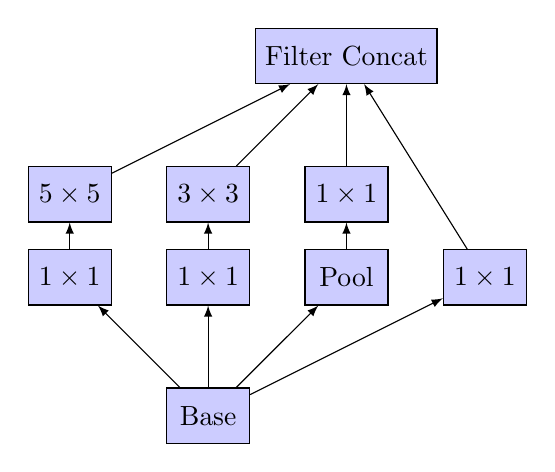
\begin{tikzpicture}[node distance=1.6cm]

    \node (concat) [block] {Filter Concat};

    \node (211) [block, below of=concat] {$1\times1$};
    \node (233) [block, left of=211] {$3\times3$};
    \node (255) [block, left of=233] {$5\times5$};


    \node (pool) [block, below of=211, node distance=3em] {Pool};

    \node (1111) [block, left of=pool] {$1\times1$};
    \node (1112) [block, left of=1111] {$1\times1$};
    \node (1113) [block, right of=pool] {$1\times1$};

    \node (base) [block, below of=1111] {Base};

    
    \draw[arrow] (base) -- (1111);
    \draw[arrow] (base) -- (1112);
    \draw[arrow] (base) -- (pool);
    \draw[arrow] (base) -- (1113);

    \draw[arrow] (pool) -- (211);
    \draw[arrow] (1111) -- (233);
    \draw[arrow] (1112) -- (255);
    \draw[arrow] (1113) -- (concat);

    \draw[arrow] (255) -- (concat);
    \draw[arrow] (233) -- (concat);
    \draw[arrow] (211) -- (concat);

    

\end{tikzpicture}
